% Vietnamese translation for OI Public Library
% Source-PDF: IOI中国国家候选队论文/2002/杨旻旻.pdf
\documentclass[11pt]{article}
\usepackage{oipl-vn}
\usepackage{tikz}

\title{Phương pháp xây dựng: con đường ngắn nhất để giải bài}
\author{Yang Minmin}
\date{}

\newcommand{\vect}[1]{\left\langle #1\right\rangle}

\begin{document}
\maketitle

\origtitle{Constructive method: the shortest path to solving problems}
\sourcepath{IOI China candidate team papers / 2002 / Yang Minmin.pdf}

\section{Mở đầu}

Bài giảng này xoay quanh \term{phương pháp xây dựng}: một kiểu suy nghĩ trong
đó ta trực tiếp dựng ra đối tượng thỏa yêu cầu, hoặc dựng ra phản ví dụ để phủ
định một kết luận; đôi khi ta cũng dựng gián tiếp một quan hệ tương ứng để
chuyển bài toán về dạng cần thiết.

Nội dung chính gồm ba phần:
\begin{itemize}
  \item phương pháp xây dựng và các đặc điểm của nó;
  \item những dạng xây dựng thường dùng;
  \item ưu điểm và nhược điểm của phương pháp xây dựng.
\end{itemize}

\section{Phương pháp xây dựng và đặc điểm}

Phương pháp xây dựng không phải là thử bừa đơn giản, cũng không phải là may
mắn nhất thời. Điều kiện để dùng nó là bài toán có tính tồn tại: ta cần chứng
minh hoặc tìm ra một đối tượng thỏa điều kiện nào đó. Vì vậy phương pháp này
đặc biệt thích hợp với các bài thi lập trình yêu cầu tìm một nghiệm khả thi
duy nhất.

Ưu điểm của phương pháp xây dựng là độ phức tạp thời gian và bộ nhớ thường
nhỏ, chương trình cũng thường ngắn và trực tiếp. Nhược điểm là độ phức tạp tư
duy cao: phần khó nằm ở việc tìm ra cách dựng đúng.

Trong bài này ta xét ba dạng thường gặp:
\begin{itemize}
  \item xây dựng trực tiếp;
  \item xây dựng theo trường hợp;
  \item xây dựng bằng quy nạp.
\end{itemize}

\section{Xây dựng trực tiếp}

Xây dựng trực tiếp là cách khảo sát ngay đối tượng đích rồi dựng ra nó. Linh
hồn của phương pháp này là quá trình tìm tòi: đằng sau một lời giải xây dựng
ngắn gọn thường là rất nhiều lần thử và điều chỉnh.

Trong ứng dụng thực tế, ta thường quan sát đối tượng cần dựng, tìm các quy
luật có tính tổng quát, rồi đưa quy luật ấy vào phép dựng. Ta có thể tìm trong
những trường hợp quen thuộc, tìm trong các trường hợp đặc biệt, luôn đối chiếu
với mục tiêu, liên tục chỉnh sửa hoặc thậm chí thay đổi phương án cho đến khi
phép dựng thành công.

\subsection{Ví dụ 1: cần trục ba tay}

\paragraph{Đề bài.}
Cho ba số $p,q,n$. Cần dựng một số bộ ba thỏa bốn yêu cầu:
\begin{enumerate}
  \item Mỗi bộ ba phải có một trong hai dạng
  \[
    (i,\ i+p,\ i+p+q)\quad\text{hoặc}\quad
    (i,\ i+q,\ i+p+q).
  \]
  \item Mọi phần tử xuất hiện trong các bộ ba không vượt quá $n+p+q$.
  \item Mỗi số trong $1,2,\ldots,n+p+q$ xuất hiện nhiều nhất một lần.
  \item Các bộ ba phải phủ hết $n$ số tự nhiên $1,2,\ldots,n$.
\end{enumerate}
Giới hạn là $n\le 300000$ và $p+q\le 60000$.

\paragraph{Quan sát ban đầu.}
Rất tự nhiên ta nghĩ đến một phép dựng tham lam. Một vài ví dụ nhỏ là
\[
\begin{array}{c|c|c|c}
p=1,q=1 & p=2,q=4 & p=3,q=1 & p=1,q=3\\ \hline
(1,2,3) & (1,3,7) & (1,4,5) & (1,2,5)\\
(4,5,6) & (2,4,8) & (2,3,6) & (3,4,7)\\
(7,8,9) & (5,9,11) & (7,10,11) & (6,9,10)\\
\cdots & (6,10,12) & \cdots & (8,11,12)\\
& \cdots & & \cdots
\end{array}
\]
Từ đó dễ nảy ra cách làm sau. Giả sử đã dựng được $s$ bộ ba
\[
  (x_1,y_1,z_1),(x_2,y_2,z_2),\ldots,(x_s,y_s,z_s),
  \qquad x_1<x_2<\cdots<x_s.
\]
Lấy $r$ là số tự nhiên nhỏ nhất chưa xuất hiện trong $s$ bộ ba ấy.
Nếu $r+p$ chưa xuất hiện, dựng bộ ba tiếp theo là
\[
  (x_{s+1},y_{s+1},z_{s+1})=(r,\ r+p,\ r+p+q).
\]
Nếu $r+p$ đã xuất hiện, dựng
\[
  (x_{s+1},y_{s+1},z_{s+1})=(r,\ r+q,\ r+p+q).
\]

Cách này bị ví dụ $p=3,q=2$ bác bỏ ngay:
\[
  (1,4,6),\qquad (2,5,7),\qquad (3,?,8).
\]
Ở dấu hỏi, cả $5$ lẫn $6$ đều đã xuất hiện. Nhưng nếu đổi vai trò hai tham số,
tức xét $p=2,q=3$, ta lại có thể đi tiếp:
\[
  (1,3,6),\qquad (2,4,7),\qquad (5,8,10),\qquad (9,11,14),\ldots
\]
Điều này gợi ý rằng cách điền trên cần giả thiết $p\le q$. Khi $p>q$, ta đổi
hai giá trị $p,q$ trước rồi mới áp dụng phép dựng. Đây mới chỉ là phỏng đoán,
cần được kiểm nghiệm và chứng minh.

\paragraph{Phép dựng hoàn chỉnh.}
Trước hết, nếu $p>q$ thì hoán đổi hai giá trị $p,q$; do hai dạng bộ ba đối
xứng theo $p$ và $q$, việc này không ảnh hưởng đến khả năng dựng nghiệm.
Sau đó lặp lại quy tắc:
\begin{enumerate}
  \item Giả sử đã dựng được $s$ bộ ba
  $(x_1,y_1,z_1),\ldots,(x_s,y_s,z_s)$ với
  $x_1<x_2<\cdots<x_s$.
  \item Lấy $r$ là số tự nhiên nhỏ nhất chưa xuất hiện trong các bộ ba đã dựng.
  \item Nếu $r+p$ chưa xuất hiện, thêm bộ ba $(r,r+p,r+p+q)$.
  \item Nếu $r+p$ đã xuất hiện, thêm bộ ba $(r,r+q,r+p+q)$.
\end{enumerate}

Nhìn từ đề bài, vị trí của $p$ và $q$ có vẻ đối xứng. Vậy tại sao lại cần giả
thiết $p\le q$? Điểm then chốt là mệnh đề sau.

\paragraph{Chứng minh.}
Nếu $r+p$ đã xuất hiện thì $r+q$ nhất định chưa xuất hiện.
Giả sử ngược lại rằng cả $r+p$ và $r+q$ đều đã xuất hiện.
\begin{enumerate}
  \item Nếu $r+q=x_i+p$ với $1\le i\le s$, vì $q\ge p$ nên
  \[
    r=x_i+p-q\le x_i.
  \]
  Điều này mâu thuẫn với việc $r$ là số tự nhiên nhỏ nhất chưa xuất hiện trong
  $s$ bộ ba đầu.
  \item Nếu $r+q=x_i+p+q$ với $1\le i\le s$, thì $r=x_i+p$.
  Vì $r$ chưa xuất hiện, tại bước dựng bộ ba thứ $i$ lẽ ra $x_i+p$ chưa xuất
  hiện và phải được chọn ưu tiên. Mâu thuẫn.
\end{enumerate}
Do đó khi nhánh thứ hai xảy ra, $r+q$ là vị trí hợp lệ để điền. Ví dụ này cho
thấy một phép dựng có thể cần rất nhiều lần thử trước khi lộ ra điều kiện đúng.

\section{Nhiều phép dựng bổ trợ nhau}

\subsection{Ví dụ 2: tô màu các đoạn}

\paragraph{Đề bài.}
Cho $n$ đoạn thẳng. Biết rằng mọi điểm của $[t_0,t_1]$ đều được ít nhất một
đoạn phủ. Hãy tô màu một số đoạn sao cho tổng độ dài phần chỉ được đúng một
đoạn đã tô phủ không nhỏ hơn
\[
  \frac{2}{3}(t_1-t_0).
\]

Hình sau minh họa ba đoạn được tô; phần đậm là phần chỉ được đúng một đoạn tô
phủ.
\[
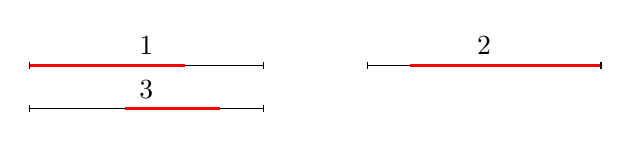
\begin{tikzpicture}[x=1.1cm,y=0.55cm]
  \draw (0,2) -- (2.7,2);
  \draw[red,very thick] (0,2) -- (1.8,2);
  \draw (0,1) -- (2.7,1);
  \draw[red,very thick] (1.1,1) -- (2.2,1);
  \draw (3.9,2) -- (6.6,2);
  \draw[red,very thick] (4.4,2) -- (6.6,2);
  \node at (1.35,2.45) {$1$};
  \node at (5.25,2.45) {$2$};
  \node at (1.35,1.45) {$3$};
  \foreach \x/\y in {0/2,2.7/2,0/1,2.7/1,3.9/2,6.6/2}
    \draw (\x,\y-0.08) -- (\x,\y+0.08);
\end{tikzpicture}
\]

\paragraph{Chuẩn hóa các đoạn.}
Gọi các đoạn là
\[
  [a_1,b_1],[a_2,b_2],\ldots,[a_n,b_n],
  \qquad a_1\le a_2\le\cdots\le a_n.
\]
Ta thực hiện các phép xóa trong trường hợp vẫn bảo đảm không mất nghiệm, với
mục tiêu làm quan hệ giữa các đoạn đơn giản hơn. Sau khi chuẩn hóa, có thể giả
sử:
\[
  a_1<a_2<\cdots<a_n,
\]
\[
  b_1<b_2<\cdots<b_n,
\]
và
\[
  b_1<a_3<b_2,\quad b_2<a_4<b_3,\quad \ldots,\quad
  b_{n-2}<a_n<b_{n-1}.
\]

\paragraph{Ba cách tô.}
Ta xét đồng thời ba phép dựng:
\begin{enumerate}
  \item Tô các đoạn có chỉ số lẻ:
  \[
    [a_1,b_1],[a_3,b_3],[a_5,b_5],\ldots
  \]
  Khi đó độ dài phần chỉ được đúng một đoạn tô phủ là
  \[
    l_1=\sum_{\substack{1\le i\le n\\ i\ \text{lẻ}}}(b_i-a_i).
  \]
  \item Tô các đoạn có chỉ số chẵn:
  \[
    [a_2,b_2],[a_4,b_4],[a_6,b_6],\ldots
  \]
  Khi đó
  \[
    l_2=\sum_{\substack{1\le i\le n\\ i\ \text{chẵn}}}(b_i-a_i).
  \]
  \item Tô toàn bộ $n$ đoạn. Khi đó phần chỉ được đúng một đoạn tô phủ có độ
  dài
  \[
    l_3=a_2-a_1+\sum_{i=2}^{n-1}(a_{i+1}-b_{i-1})+b_n-b_{n-1}.
  \]
\end{enumerate}

Chỉ cần chứng minh: nếu
\[
  l_1,l_2<\frac{2}{3}(t_1-t_0),
\]
thì nhất định
\[
  l_3\ge \frac{2}{3}(t_1-t_0).
\]
Ta biến đổi
\[
  l_3=\sum_{i=1}^{n}a_i-\sum_{i=1}^{n}b_i+2(b_n-a_1),
\]
trong khi
\[
  l_1+l_2=\sum_{i=1}^{n}(b_i-a_i)
          =\sum_{i=1}^{n}b_i-\sum_{i=1}^{n}a_i.
\]
Do các đoạn phủ toàn bộ $[t_0,t_1]$, ta có $b_n\ge t_1$ và $a_1\le t_0$.
Suy ra
\[
\begin{aligned}
  l_3
  &\ge 2(t_1-t_0)-(l_1+l_2)\\
  &>2(t_1-t_0)-\frac{4}{3}(t_1-t_0)
   =\frac{2}{3}(t_1-t_0).
\end{aligned}
\]
Vậy trong $l_1,l_2,l_3$ nhất định có một giá trị không nhỏ hơn
$\frac{2}{3}(t_1-t_0)$, và ba phép dựng trên bảo đảm tìm được cách tô hợp lệ.

Điểm đặc biệt của bài này là ta không cố đưa ra ngay một phép dựng luôn đúng.
Thay vào đó, ta dựng nhiều phương án cùng lúc và chứng minh ít nhất một phương
án phải thành công. Một phép dựng thất bại có thể tạo điều kiện để phép dựng
khác thành công:
\[
\begin{array}{rcl}
\text{dựng A thất bại}\\
\text{dựng B thất bại} & \Longrightarrow & \text{dựng D thành công},\\
\text{dựng C thất bại}
\end{array}
\]

\section{Xây dựng theo trường hợp}

Khi bài toán có nhiều khả năng xảy ra và khó xử lý thống nhất, ta phân loại
toàn bộ các tình huống có thể, giải riêng từng loại rồi ghép các kết luận lại.
Đó là tư tưởng phân loại.

Xây dựng theo trường hợp là sự kết hợp giữa tư tưởng phân loại và phương pháp
xây dựng. Quy trình thường là
\[
\text{phân tích tính chất bài toán}
\Longrightarrow
\text{phân loại bài toán}
\Longrightarrow
\text{xây dựng cho từng loại}
\Longrightarrow
\text{ghép thành lời giải}.
\]
Các tiêu chuẩn phân loại quen thuộc đều có thể dùng: phân loại theo lớp dư
như chẵn lẻ, theo kích thước dữ liệu, theo khái niệm trong đề, hoặc theo sự
thay đổi của tham số.

\subsection{Ví dụ 3: đi qua bàn cờ}

\paragraph{Đề bài.}
Cho một hình vuông $n\times n$. Một người xuất phát từ ô $(x,y)$. Hãy tìm một
đường đi qua mỗi ô đúng một lần.

Với $n=4$, $x=2$, $y=2$, một đường đi dạng gấp khúc ngoằn ngoèo có thể minh
họa như sau.
\[
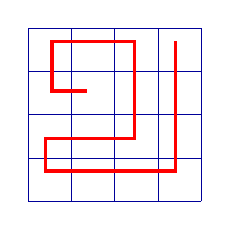
\begin{tikzpicture}[scale=0.55]
  \draw[step=1,blue!60!black] (0,0) grid (4,4);
  \draw[red,very thick]
    (3.4,3.7) -- (3.4,0.7) -- (0.4,0.7) -- (0.4,1.45)
    -- (2.45,1.45) -- (2.45,3.7) -- (0.55,3.7)
    -- (0.55,2.55) -- (1.35,2.55);
\end{tikzpicture}
\]
Ta muốn đường đi càng đơn giản càng tốt, số lần rẽ càng ít càng tốt; dạng tự
nhiên là một đường gấp khúc ngoằn ngoèo. Đặc điểm quan trọng là hướng của
đường đi tại biên phụ thuộc vào tính chẵn lẻ của $n,x,y$.

Một khi tính chẵn lẻ của $n,x,y$ đã xác định, cách đường đi gặp biên cũng được
xác định. Vì thế ta phân loại theo các tính chẵn lẻ ấy.

\paragraph{Trường hợp $n$ chẵn.}
Không mất tính tổng quát, có thể giả sử $x,y$ đều lẻ; nếu không, ta xoay hoặc
lật bàn cờ một cách thích hợp. Khi đó có thể dùng đường ngoằn ngoèo theo từng
dải để đi qua toàn bộ bàn cờ.

\[
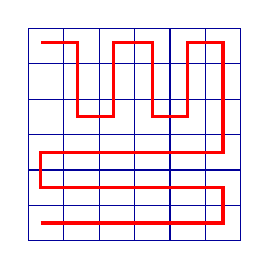
\begin{tikzpicture}[scale=0.45]
  \draw[step=1,blue!60!black] (0,0) grid (6,6);
  \draw[red,very thick]
    (0.35,0.5) -- (5.5,0.5) -- (5.5,1.5) -- (0.35,1.5)
    -- (0.35,2.5) -- (5.5,2.5) -- (5.5,5.6)
    -- (4.5,5.6) -- (4.5,3.5) -- (3.5,3.5)
    -- (3.5,5.6) -- (2.4,5.6) -- (2.4,3.5)
    -- (1.4,3.5) -- (1.4,5.6) -- (0.35,5.6);
\end{tikzpicture}
\]

\paragraph{Trường hợp $n$ lẻ và $x,y$ cùng tính chẵn lẻ.}
Không mất tính tổng quát, có thể giả sử $x,y$ đều chẵn; nếu không, ta cũng
xoay hoặc lật bàn cờ. Lúc này vẫn có thể dựng một đường gấp khúc ngoằn ngoèo
tương tự, chỉ khác cách nối ở gần điểm xuất phát và ở biên.

\[
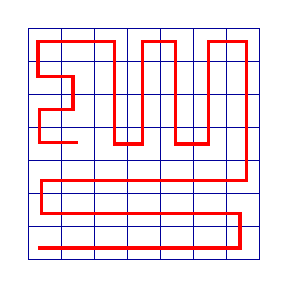
\begin{tikzpicture}[scale=0.42]
  \draw[step=1,blue!60!black] (0,0) grid (7,7);
  \draw[red,very thick]
    (0.3,0.35) -- (6.4,0.35) -- (6.4,1.4) -- (0.4,1.4)
    -- (0.4,2.4) -- (6.6,2.4) -- (6.6,6.6)
    -- (5.45,6.6) -- (5.45,3.5) -- (4.45,3.5)
    -- (4.45,6.6) -- (3.45,6.6) -- (3.45,3.5)
    -- (2.6,3.5) -- (2.6,6.6) -- (0.3,6.6)
    -- (0.3,5.55) -- (1.35,5.55) -- (1.35,4.55)
    -- (0.35,4.55) -- (0.35,3.55) -- (1.5,3.55);
\end{tikzpicture}
\]

\paragraph{Trường hợp $n$ lẻ và $x,y$ khác tính chẵn lẻ.}
Bài toán vô nghiệm. Tô bàn cờ bằng hai màu đen trắng. Vì $n$ lẻ, tổng số ô là
lẻ và một màu nhiều hơn màu kia đúng một ô. Mọi đường đi qua mỗi ô đúng một
lần có số ô lẻ, nên nếu bắt đầu ở màu trắng thì phải kết thúc ở màu đen, và
số ô trắng bằng số ô đen trên đường đi. Nhưng trên bàn cờ $n$ lẻ, số ô của
hai màu không bằng nhau. Mâu thuẫn.

Ở bài này, tiêu chuẩn phân loại không xuất hiện từ hư không. Nó đến từ đặc
tính của đường gấp khúc ngoằn ngoèo: khi đường đi gặp biên, hành vi của nó
thay đổi theo tính chẵn lẻ. Do đó tiêu chuẩn phân loại gắn chặt với chính
phương pháp xây dựng đã chọn.

\section{Xây dựng bằng quy nạp}

Quy nạp ở đây là quy nạp toán học. Phương pháp này được dùng rất nhiều vì chỉ
từ hữu hạn bước mà đi qua được vô hạn trường hợp. Nó có nhiều biến thể như quy
nạp mạnh, quy nạp nhiều điểm xuất phát, quy nạp theo đường cong.

Xây dựng bằng quy nạp dùng tư tưởng quy nạp để tạo ra đối tượng cần dựng. Một
dạng rất phổ biến trong thi lập trình là ``quy nạp thông thường cộng với xây
dựng''. Các bước tổng quát là:
\[
\begin{array}{c}
\text{dựng trường hợp } i=1,\\[0.3em]
\text{giả sử đã dựng được trường hợp } i=j
\text{ rồi dựng trường hợp } i=j+1,\\[0.3em]
\text{dùng quy nạp để mở rộng đến } i=n.
\end{array}
\]

\subsection{Ví dụ 4: sắp lịch thi đấu, bài toán thứ nhất}

\paragraph{Đề bài.}
Có $2^m$ đấu thủ. Mỗi ngày có thể sắp một số trận, và mỗi đấu thủ trong một
ngày chỉ được tham gia một trận. Hãy đưa ra một lịch thi đấu sao cho trong
$2^m-1$ ngày, mọi cặp đấu thủ đều đã gặp nhau ít nhất một lần.

Ta thiết kế lịch thành một ma trận $2^m\times 2^m$ như sau, bỏ hàng tiêu đề
ngày, và ký hiệu là $P_m$:
\[
\begin{array}{c|ccccc}
& \text{ngày 1} & \text{ngày 2} & \cdots & \text{ngày }2^m-1
& \text{ngày }2^m\\ \hline
\text{đấu thủ }1\\
\text{đấu thủ }2\\
\vdots\\
\text{đấu thủ }2^m-1\\
\text{đấu thủ }2^m
\end{array}
\]
Cột đầu tiên chỉ chứa chính số hiệu đấu thủ; các cột còn lại cho biết đối thủ
tương ứng từng ngày. Với cách hiểu đó, ma trận có các tính chất:
\begin{enumerate}
  \item Phần tử ở hàng $i$, cột đầu tiên là $i$.
  \item Tập các số trên hàng $i$ là $\{1,2,3,\ldots,2^m\}$.
  \item Tập các số trên cột $j$ là $\{1,2,3,\ldots,2^m\}$.
  \item Nếu phần tử ở hàng $i$, cột $j$ là $k$, thì phần tử ở hàng $k$, cột
  $j$ là $i$.
\end{enumerate}

Tư tưởng quy nạp là trước hết dựng $P_m$, rồi từ $P_m$ dựng $P_{m+1}$.
Ma trận $P_{m+1}$ có kích thước $2^{m+1}\times 2^{m+1}$, gợi ý chia nó thành
bốn khối $2^m\times 2^m$:
\[
\begin{array}{|c|c|}
\hline
A & B\\ \hline
C & D\\ \hline
\end{array}
\]
Khi $P_m$ đã được điền, đặt
\[
  A=D=P_m,\qquad B=C=P_m+2^m,
\]
trong đó $P_m+2^m$ nghĩa là cộng $2^m$ vào mọi phần tử của $P_m$. Do đó
\[
  P_{m+1}=
  \begin{pmatrix}
    P_m & P_m+2^m\\
    P_m+2^m & P_m
  \end{pmatrix}.
\]
Dễ kiểm tra rằng ma trận thu được vẫn thỏa bốn tính chất trên. Từ ma trận ấy
ta đọc được lịch thi đấu cần tìm.

\subsection{Ví dụ 4: sắp lịch thi đấu, bài toán thứ hai}

\paragraph{Đề bài.}
Có $2^n$ đấu thủ tham gia. Khi hai đấu thủ gặp nhau, người mạnh hơn luôn
thắng, và không có hai đấu thủ mạnh ngang nhau. Mỗi ngày, mỗi đấu thủ nhiều
nhất gặp một đối thủ. Hãy đưa ra một lịch thi đấu sao cho trong
\[
  \frac{n(n+1)}{2}
\]
ngày có thể xác định thứ tự mạnh yếu của toàn bộ đấu thủ.

Để tiện trình bày, viết $A>B$ nếu đấu thủ $A$ mạnh hơn đấu thủ $B$.
Trước hết thử quy nạp thông thường. Giả sử kết luận đúng với $n$, xét
$n+1$. Có $2^{n+1}$ đấu thủ, chia thành hai nhóm $A$ và $B$, mỗi nhóm
$2^n$ người. Theo giả thiết quy nạp, chỉ cần $\frac{n(n+1)}{2}$ ngày để xác
định thứ tự trong từng nhóm:
\[
  A_1>A_2>A_3>\cdots>A_{2^n},
  \qquad
  B_1>B_2>B_3>\cdots>B_{2^n}.
\]
Ta còn phải hợp nhất hai dãy này trong
\[
  \frac{(n+1)(n+2)}{2}-\frac{n(n+1)}{2}=n+1
\]
ngày. Đây là bước then chốt và cũng là nút thắt của bài toán.

Nói cách khác, bài toán chuyển thành: biết hai dãy đã sắp
\[
  A_1>A_2>\cdots>A_{2^n},\qquad
  B_1>B_2>\cdots>B_{2^n},
\]
hãy xác định thứ tự của $2^{n+1}$ người trong $n+1$ ngày.
Sau nhiều lần thử, ta thấy quy nạp thông thường không đủ mạnh ở bước
``tách rồi hợp''. Một kỹ thuật quen thuộc của quy nạp toán học là
\term{tăng cường mệnh đề}.

\paragraph{Mệnh đề tăng cường.}
Với $k+l=2^n$, trong đó $k,l,n$ là các số nguyên dương, nếu đã biết
\[
  A_1>A_2>A_3>\cdots>A_k,
  \qquad
  B_1>B_2>B_3>\cdots>B_l,
\]
thì chỉ cần $n$ ngày để xác định thứ tự mạnh yếu của $2^n$ đấu thủ này.

Mệnh đề tăng cường vẫn giải được bằng xây dựng quy nạp.

Khi $n=1$, ta có $k=l=1$. Sắp trận $A_1$ đấu $B_1$ là đủ, kết luận hiển
nhiên đúng.

Giả sử với $n$ đã có cách sắp lịch, xét trường hợp $n+1$. Không mất tính tổng
quát, giả sử $k\le l$ và $k+l=2^{n+1}$. Ngày đầu tiên, sắp các trận
\[
\begin{array}{c|cccc|c}
\text{nhóm A} & A_1 & A_2 & \cdots & A_k & \text{yếu dần}\\ \hline
\text{nhóm B} & B_{2^n} & B_{2^n-1} & \cdots & B_{2^n-k+1}
& \text{mạnh dần}
\end{array}
\]
tức là $A_i$ gặp $B_{2^n-i+1}$ với $1\le i\le k$.

Gọi $A_j$ là đấu thủ có chỉ số nhỏ nhất trong nhóm $A$ thua đối thủ của mình.
Khi đó $A_1,A_2,\ldots,A_{j-1}$ đều thắng, còn
$A_j,A_{j+1},\ldots,A_k$ đều thua. Ta suy ra được hai chuỗi quan hệ:
\[
  A_1>A_2>\cdots>A_{j-1}>
  B_{2^n-j+2}>B_{2^n-j+3}>\cdots>B_{2^n}> \cdots >B_l,
\]
\[
  B_1>B_2>\cdots>B_{2^n-j+1}>
  A_j>A_{j+1}>\cdots>A_k.
\]

Chia $2^{n+1}$ đấu thủ thành hai nhóm, mỗi nhóm $2^n$ người:
\[
\begin{aligned}
\text{nhóm mạnh:}\quad
&A_1>A_2>\cdots>A_{j-1},\quad
  B_1>B_2>\cdots>B_{2^n-j+1},\\
\text{nhóm yếu:}\quad
&A_j>A_{j+1}>\cdots>A_k,\quad
  B_{2^n-j+2}>B_{2^n-j+3}>\cdots>B_l.
\end{aligned}
\]
Dễ thấy mọi người trong nhóm mạnh đều mạnh hơn mọi người trong nhóm yếu.
Theo giả thiết quy nạp, thứ tự bên trong mỗi nhóm chỉ cần $n$ ngày nữa, và
hai nhóm có thể thi song song. Vì toàn bộ nhóm mạnh đứng trước toàn bộ nhóm
yếu, thứ tự chung cũng được xác định. Cộng với ngày đầu tiên, tổng cộng cần
$n+1$ ngày; vậy mệnh đề tăng cường đúng với $n+1$.

Khi mệnh đề tăng cường đã đúng, kết luận ban đầu cũng đúng. Quay lại bài toán
gốc, sau khi biết hai dãy
\[
  A_1>A_2>\cdots>A_{2^n},\qquad
  B_1>B_2>\cdots>B_{2^n},
\]
ta chỉ cần $n+1$ ngày để hợp nhất chúng. Tổng số ngày là
\[
  \frac{n(n+1)}{2}+(n+1)=\frac{(n+1)(n+2)}{2},
\]
nên trường hợp $n+1$ cũng hoàn thành.

Hai bài lịch thi đấu trên đều là ví dụ điển hình của xây dựng quy nạp. Bài
thứ nhất chuyển từ $m$ sang $m+1$ rất trực tiếp; bài thứ hai phải tăng cường
mệnh đề và dùng quy nạp hai lần. Tăng cường mệnh đề là một kỹ thuật toán học
quan trọng: khi kết luận được làm mạnh hơn, giả thiết quy nạp cũng mạnh hơn,
và chính điều đó mở đường cho phép dựng.

\section{Kết luận}

Phương pháp xây dựng thường đem lại lời giải có độ phức tạp thấp và cài đặt
gọn, nhưng đòi hỏi khả năng quan sát và biến đổi cao. Trong quá trình xây
dựng, ta cần kết hợp nhiều công cụ toán học: thử các trường hợp đặc biệt,
phân loại, chứng minh điều kiện đúng, dựng nhiều phương án bổ trợ nhau, và
khi cần thì tăng cường mệnh đề quy nạp.

\end{document}
